% Relatorio do Monte Carlo da chuva (Rahardjo et al. 2007 + Vargas Ceron et al. 2025). Para refazer:
%   python3 -I figuras_relatorio.py   (figuras em figs/; imprime as linhas das tabelas e cada numero do texto com
%                                      o arquivo de onde sai)
%   pdflatex relatorio_chuva.tex      (duas vezes)
\documentclass[11pt,a4paper]{article}
\usepackage[T1]{fontenc}\usepackage[utf8]{inputenc}\usepackage[brazilian]{babel}\usepackage{lmodern}
\usepackage[margin=2.2cm]{geometry}\usepackage{booktabs}\usepackage{graphicx}\usepackage{caption}
\usepackage{float}\usepackage[hidelinks]{hyperref}\usepackage{amsmath}\usepackage{amssymb}\usepackage{microtype}
\usepackage{array}
\captionsetup{font=small}
% mais floats por pagina de texto e paginas so de floats so quando cheias
\renewcommand{\topfraction}{0.9}\renewcommand{\bottomfraction}{0.8}\renewcommand{\textfraction}{0.07}
\renewcommand{\floatpagefraction}{0.75}
\graphicspath{{figs/}}
\author{SlopeRandomFieldRefinement\\ \small(\texttt{rahardjo.cpp}, \texttt{montecarlo.cpp}, \texttt{form\_variaveis.py}, \texttt{rebaixamento\_mc.cpp})}
\title{Monte Carlo da chuva no talude de Rahardjo et al.\ (2007) com o método estocástico de Vargas Ceron et al.\
(2025): validação, escolhas e campanha no fermi}
\date{14 de novembro de 2026}
\begin{document}\maketitle

\section{Objetivo e plano}\label{sec:objetivo}
O objetivo é a probabilidade de ruptura $P_f$ de um talude sob chuva, com a resistência e a permeabilidade do solo como
campos aleatórios. O problema da chuva é o talude homogêneo de Rahardjo et al.\ (2007), com $H = 10$~m a $45^\circ$ e o
solo $f_{50,-5}$. O método estocástico é o de Vargas Ceron et al.\ (2025): $c'$, $\varphi'$ e $k_s$ log-normais, gerados
por Karhunen--Loève, e Monte Carlo. A campanha repete as Seções 6.1 a 6.5 do Ceron, com a intensidade da chuva no lugar
da altura do rebaixamento (6.5). Cada parte tem a sua referência: o Rahardjo valida a física da chuva (o $FS$
determinístico no tempo) e o Ceron, o método estocástico.

O plano segue a ordem deste relatório:
\begin{enumerate}
\item validar o determinístico contra a Fig.~5 do Rahardjo nos três solos (Seção~\ref{sec:validacao});
\item escolher o fator de segurança: redução da resistência (SRM) ou aumento da gravidade (GIM)
(Seção~\ref{sec:gimsrm});
\item escolher a intensidade de referência e conferir o Monte Carlo com pilotos de 8 a 10 realizações
(Seção~\ref{sec:intensidade});
\item estimar $P_f$ pelo FORM com variáveis aleatórias e ver o que o FORM pediria com campos (Seção~\ref{sec:form});
\item testar a amostragem por importância no rebaixamento do Ceron, onde há um Monte Carlo direto para comparar
(Seção~\ref{sec:ai});
\item rodar a campanha no fermi (Seção~\ref{sec:fermi}).
\end{enumerate}
Os passos 1 a 4 estão feitos. O passo 5 está rodando no PC e vai para o fermi. A campanha da chuva está pronta para
submeter. As figuras e as tabelas saem de
\texttt{relatorio/figuras\_relatorio.py}. Ele lê os arquivos gravados pelos programas (logs do \texttt{SlopeRahardjo},
CSVs do \texttt{SlopeRainMonteCarlo} e o \texttt{form.json} do \texttt{form\_variaveis.py}) e imprime cada número do
texto com o arquivo de onde ele sai. O Apêndice~\ref{sec:arquivos} lista os arquivos.

\section{Modelo}\label{sec:modelo}
\subsection{Talude e solos}
O talude é o da Fig.~2 do Rahardjo (Fig.~\ref{fig:geometria}). O nível d'água inicial fica 5~m abaixo do pé e sobe
$7^\circ$ para dentro do maciço. Acima dele a pressão é hidrostática negativa, com a sucção limitada a 75~kPa, como no
artigo. Os três solos da Tabela~1 do artigo (Tab.~\ref{tab:solos}) só diferem em $a$ e $k_s$. Os outros dados são comuns:
$c' = 10$~kPa, $\varphi' = \varphi^b = 26^\circ$ e $\gamma = 20$~kN/m$^3$ acima e abaixo do nível. O módulo $E = 20$~MPa e
$\nu = 0{,}3$ não estão no artigo e não mudam o $FS$.

\begin{figure}[htbp]\centering
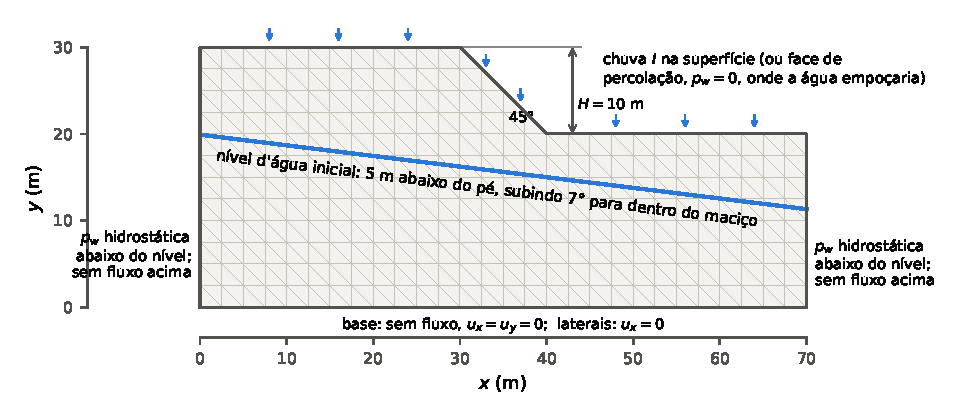
\includegraphics[width=\linewidth]{fig_geometria.pdf}
\caption{Talude da Fig.~2 de Rahardjo et al.\ (2007), contornos da percolação e do deslocamento, nível d'água inicial e a
malha do transiente do Monte Carlo (\texttt{TriGMesh(2)}, 560 triângulos).}\label{fig:geometria}
\end{figure}

\begin{table}[htbp]\centering\footnotesize
\caption{Solos da Tabela~1 de Rahardjo et al.\ (2007): curva de retenção de Fredlund--Xing com $C(\psi) = 1$ e
permeabilidade $k_w = k_s\Theta^p$, $\Theta = \theta_w/\theta_s$. O nome $f_{a,e}$ junta $a$ (kPa) e o expoente de $k_s$
(m/s).}\label{tab:solos}
\begin{tabular}{lrrrrrrr}\toprule
solo & $a$ (kPa) & $n$ & $m$ & $\theta_s$ & $k_s$ (m/s) & $k_s$ (mm/h) & $p$ \\\midrule
$f_{10,-4}$ & 10 & 1 & 1 & 0,45 & $10^{-4}$ & 360 & 4 \\
$f_{50,-5}$ & 50 & 1 & 1 & 0,45 & $10^{-5}$ & 36 & 4 \\
$f_{100,-6}$ & 100 & 1 & 1 & 0,45 & $10^{-6}$ & 3,6 & 4 \\
\bottomrule\end{tabular}\end{table}

\subsection{Transiente da chuva}
O transiente (\texttt{RainTransient}) segue as hipóteses do SEEP/W do artigo:
\begin{itemize}
\item esqueleto rígido ($u = 0$) e ar passivo ($p_a = 0$): só a equação de Richards para $p_w$, no material
\texttt{TPZMatUnsaturatedUPwPa} sem acoplamento;
\item Euler implícito com passo de 0,1~h e armazenamento concentrado;
\item na superfície (crista, face e terreno depois do pé), a chuva $I$ por metro de superfície. Onde a água empoçaria ($p_w > 0$), a
superfície vira face de percolação, com $p_w = 0$. Um nó da face volta ao fluxo da chuva se absorver mais do que ela. O
conjunto de nós da face é corrigido dentro de cada passo até se repetir;
\item nas laterais, $p_w$ hidrostática abaixo do nível inicial; sem fluxo acima dele e na base;
\item chuva por 24~h. O \texttt{rahardjo.cpp} segue até 48~h, com o $FS$ de hora em hora. O Monte Carlo para no último
instante pedido (24~h).
\end{itemize}

\subsection{Fator de segurança}
O $FS$ é o da redução da resistência (SRM, \texttt{UnsatAnalysis::SRMArcLength}). As pressões do instante ficam
congeladas: $p_w$ vai da malha do transiente para a do fator por interpolação linear no triângulo que contém cada nó. A
resistência é Mohr--Coulomb associado ($\psi = \varphi'$) em tensão efetiva com $\chi = \tan\varphi^b/\tan\varphi'$, isto
é, a parcela $(u_a - u_w)\tan\varphi^b$ da Eq.~5 do artigo (aqui $\chi = 1$). O caminho tem duas partes:
\begin{enumerate}
\item peso: $\lambda$ de 0 a 1 com $F = 1$, a partir do estado sem tensões, em incrementos de Newton. Se o talude não fica
em pé com a resistência real ($FS < 1$), o peso recomeça com $F = 0{,}5$ (resistência dobrada) e, se preciso,
$F = 0{,}25$;
\item caminho em $F$ por \emph{arc-length} cilíndrico, o mesmo do GIM, com a carga tangente $-\partial R/\partial F$ por
diferença finita. Só os pontos plásticos contribuem para essa carga. Com nenhum ou poucos pontos plásticos, o preditor
pediria um salto de $F$ maior que 25\%. Então o passo é vertical: Newton com $F$ 10\% maior, e metade do aumento quando o
Newton não converge.
\end{enumerate}
O caminho termina no patamar ($F$ cresce menos de 0,001 num passo) e o $FS$ é o maior $F$ dele. Como $c'$ e
$\tan\varphi'$ são divididos por $F$, a parcela da sucção cai junto: é o $\tan\varphi^b/F$ do método de Bishop do
SLOPE/W, usado pelo artigo. No GIM (Seção~\ref{sec:gimsrm}), $\lambda$ multiplica o peso e a poropressão positiva, com a
sucção fixa; $\Gamma$ é o $\lambda$ do colapso.

\subsection{Malhas}
A \texttt{TriGMesh} é estruturada: passo $H$, cada retângulo em dois triângulos, a cunha da face num triângulo só e $K$
refinamentos uniformes (lado $H/2^K$).
\begin{itemize}
\item Transiente: \texttt{TriGMesh(3)} (lado de 1,25~m, 2240 triângulos) no \texttt{rahardjo.cpp}. No Monte Carlo,
\texttt{TriGMesh(2)} (2,5~m, 560 triângulos).
\item Fator: \texttt{TriGMesh(1)} (5~m) e 4 níveis de refinamento $h$ nos triângulos com
$\sqrt{J_2(\varepsilon_p)} \geq 0{,}1$ do maior. O refinamento é refeito do zero em cada instante, até o lado de
$5/2^4 \approx 0{,}31$~m na banda. Deslocamento quadrático; de 3902 a 7178 equações no último nível (logs do
\texttt{rahardjo.cpp}).
\end{itemize}
O Monte Carlo com \texttt{TriGMesh(3)} no transiente dá $FS = 2{,}0975$ em 0~h e 1,0335 em 24~h (f50, 36~mm/h). O
\texttt{rahardjo.cpp} dá 2,0975 e 1,0346. A diferença em 24~h ($-0{,}10\%$) vem da sequência de passos de tempo: o
\texttt{rahardjo.cpp} para a cada 0,25~h para gravar a animação, o que parte alguns passos de 0,1~h. Com \texttt{TriGMesh(2)} o Monte Carlo dá 2,0939
($-0{,}17\%$) e 1,0337 ($+0{,}02\%$): basta para o transiente.

\subsection{Campos aleatórios}
\begin{itemize}
\item $c'$, $\varphi'$ e $k_s$ são log-normais. O $k_s$ entra como multiplicador de média 1. As médias são 10~kPa,
$26^\circ$ e o $k_s$ do solo; os CoV, 0,3, 0,1 e 0,6 (Tabela~2 do Ceron).
\item A correlação é exponencial separável, $\exp(-|\Delta x|/L_x - |\Delta y|/L_y)$, com $L_x = 20s$~m e $L_y = 2s$~m
($s = 1$ na referência).
\item Os três campos são independentes e usam os mesmos modos: a expansão de Karhunen--Loève analítica no retângulo de
70~m $\times$ 30~m, com $M = 2000$ termos (96,4\% da variância em $s = 1$).
\item Os campos são avaliados nos pontos de integração das duas malhas: o transiente e o fator veem a mesma realização.
\item A realização $n$ usa os mesmos números aleatórios em todos os casos (semente 2025). A anisotropia é
$\alpha = k_h/k_v$, com o $k_v$ do campo.
\end{itemize}

\section{Validação determinística}\label{sec:validacao}
A Fig.~\ref{fig:validacao} e a Tab.~\ref{tab:validacao} comparam o $FS$ do \texttt{rahardjo.cpp} com as leituras da
Fig.~5 do artigo, feitas a olho ($\pm 0{,}02$). A chuva é $I = 1\,k_s$ nos três solos. As diferenças médias ficam dentro
da precisão da leitura: $+1{,}6\%$ no f10, $+0{,}7\%$ no f50 e $-0{,}2\%$ no f100; a maior é $+2{,}4\%$ (f10). O $FS$ inicial
é o mesmo nos três solos, porque a pressão inicial, a resistência e o peso não dependem do solo. Ele vale 2,0975, 1,0\%
abaixo do $F_{ini} = 2{,}118$ da Tabela~7 do artigo.


O instante do mínimo muda com o solo:
\begin{itemize}
\item f10, 360~mm/h: o $FS$ cruza 1 em 5,85~h (interpolação linear entre as horas) e fica em 0,8284 de 7 a 24~h. Nesse
patamar os 57 nós da superfície estão na face de percolação: o talude saturou até a superfície e o estado não muda mais
até o fim da chuva. Na Fig.~5a do artigo, 0,81 de 12 a 24~h.
\item f50, 36~mm/h: o mínimo, 1,0346, é o de 24~h, o fim da chuva (artigo: 1,03). Depois o $FS$ sobe.
\item f100, 3,6~mm/h: o mínimo, 1,8857, vem depois da chuva, de 32 a 34~h, 0,31\% abaixo de $FS(24\text{ h}) = 1{,}8916$.
A frente de umedecimento continua descendo depois da chuva.
\end{itemize}
Durante a chuva o $FS$ nunca sobe: de 0 a 24~h, a variação de uma hora para a seguinte é no máximo 0,0000 no f10,
$-0{,}0194$ no f50 e $-0{,}0070$ no f100. Então o menor $FS$ até o fim da chuva é o de 24~h. Por isso a campanha calcula
o $FS$ em 24~h; também em 0~h nos casos em que $c'$ ou $\varphi'$ mudam, e de 6 em 6~h na referência. A $P_f$ da campanha
é a de ruptura até o fim da chuva. No f50 determinístico o $FS$ sobe logo depois de 24~h, mas o f100 mostra que um solo
menos permeável pode ter o mínimo depois.

\begin{table}[htbp]\centering\footnotesize\setlength{\tabcolsep}{4pt}
\caption{$FS$ deste trabalho (T, \texttt{rahardjo.cpp}) e leituras da Fig.~5 do Rahardjo (R). No mínimo de T, entre
parênteses, os instantes com $FS$ até 0,0001 acima dele. Diferença: $FS_T/FS_R - 1$ nos instantes lidos.}
\label{tab:validacao}
\begin{tabular}{lrrrrrrrrrr}\toprule
& & \multicolumn{2}{c}{0~h} & \multicolumn{2}{c}{mínimo} & \multicolumn{2}{c}{48~h} & & \multicolumn{2}{c}{diferença (\%)} \\
\cmidrule(lr){3-4}\cmidrule(lr){5-6}\cmidrule(lr){7-8}\cmidrule(lr){10-11}
solo & $I$ (mm/h) & T & R & T & R & T & R & leituras & média & maior \\\midrule
$f_{10,-4}$ & 360 & 2,0975 & 2,12 & 0,8284 (7--24 h) & 0,81 & 1,5938 & 1,57 & 11 & 1,6 & 2,4 \\
$f_{50,-5}$ & 36 & 2,0975 & 2,11 & 1,0346 (24 h) & 1,03 & 1,2640 & 1,24 & 8 & 0,7 & 2,0 \\
$f_{100,-6}$ & 3{,}6 & 2,0975 & 2,11 & 1,8857 (32--34 h) & 1,89 & 1,8962 & 1,89 & 5 & $-0{,}2$ & $-0{,}6$ \\
\bottomrule\end{tabular}\end{table}

\begin{figure}[htbp]\centering
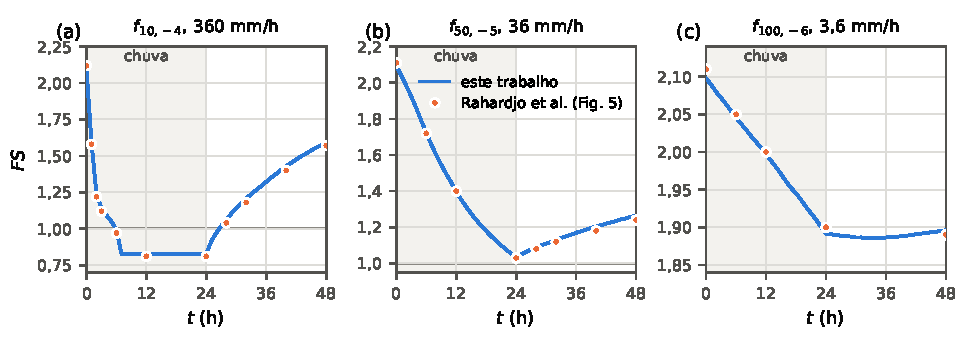
\includegraphics[width=\linewidth]{fig_validacao.pdf}
\caption{$FS(t)$ com $I = 1\,k_s$ por 24~h: este trabalho (SRM, transiente em \texttt{TriGMesh(3)}, $FS$ de hora em
hora) e as leituras da Fig.~5 de Rahardjo et al.\ (2007).}\label{fig:validacao}
\end{figure}

A Fig.~\ref{fig:estado} mostra o f50. Em 24~h o nível chega à superfície no pé e no terreno à direita, e a banda de
ruptura sai do pé e fica rasa, quase paralela à face. Em 48~h o nível desce à direita, mas continua alto sob a crista.

\begin{figure}[htbp]\centering
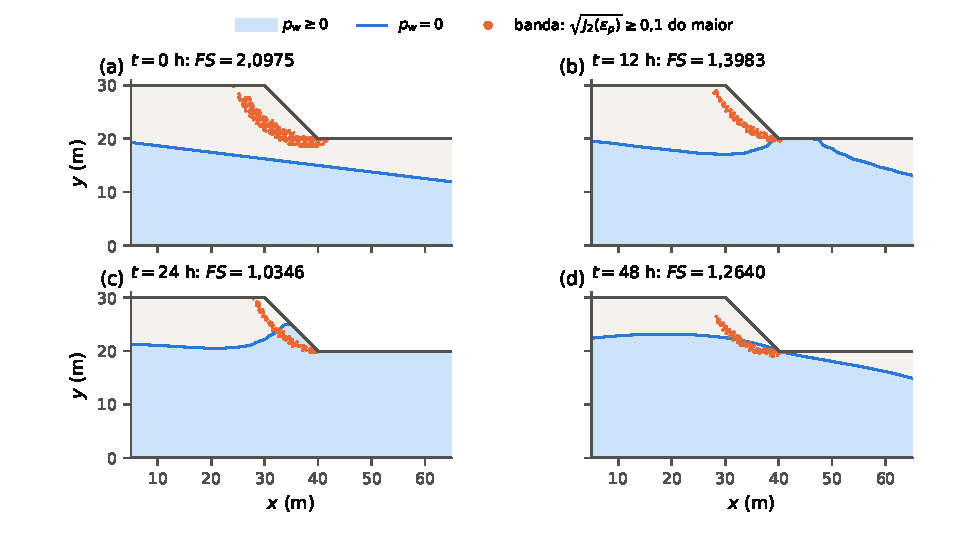
\includegraphics[width=\linewidth]{fig_estado.pdf}
\caption{Solo $f_{50,-5}$ com 36~mm/h por 24~h (o mesmo cálculo da Fig.~\ref{fig:validacao}b): zona saturada
($p_w \geq 0$) e banda de ruptura do SRM, com os pontos de integração em que $\sqrt{J_2(\varepsilon_p)}$ passa de 0,1 do
maior, em 0, 12, 24 e 48~h.}\label{fig:estado}
\end{figure}

\paragraph{Controle sem chuva.} O estado inicial, com a sucção limitada a 75~kPa, não está em equilíbrio. Sem chuva
($I = 0$, \texttt{TriGMesh(2)}), em 24~h a sucção máxima chega a 118,8~kPa e o nível sobe de 16,2/15,6/15,0~m para
16,5/15,8/15,2~m em $x = 30/35/40$~m. Mas o $FS$ vai só de 2,0939 para 2,0928 ($-0{,}054\%$): esse desvio do estado
inicial não pesa no $FS$ do f50.

\section{GIM ou SRM}\label{sec:gimsrm}
O GIM com a sucção fixa (um multiplicador da gravidade, como o $\Gamma$ do Ceron) e o SRM medem coisas diferentes longe da ruptura, e a mesma coisa
nela (Tab.~\ref{tab:gimsrm}, Fig.~\ref{fig:gimsrm}):
\begin{itemize}
\item No f50, $\Gamma = 5{,}2777$ contra $FS = 2{,}0975$ em 0~h (2,52 vezes), mas 1,0880 contra 1,0346 em 24~h. Com a
sucção fixa, aumentar o peso faz o atrito crescer junto com a carga. O GIM só vence a coesão e a parcela da sucção, que
são grandes antes da chuva.
\item No f10 os dois cruzam 1 juntos: descendo em 5,85~h (SRM) e 5,91~h (GIM), subindo em 26,57 e 26,53~h. É o
esperado: $\Gamma < 1$ e $FS < 1$ dizem a mesma coisa, que o talude não fica em pé com o peso e a resistência reais.
Então a $P_f$ contada, $\#(FS < 1)/N$, é a mesma pelos dois (Eq.~69 do Ceron), a menos do erro da malha. A média e o
CoV não são: o GIM espalha mais
(Seção~\ref{sec:intensidade}).
\item Com o refinamento, o SRM converge mais rápido (Fig.~\ref{fig:gimsrm}c). No f50 em 24~h, o último nível muda o $FS$
em 0,8\% e o $\Gamma$ em 2,8\%; em 0~h, 0,2\% e 3,3\%. O nível 0 fica 6\% (0~h) e 19\% (24~h) acima do final no SRM, e
43\% e 42\% no GIM.
\item O SRM custa o dobro: 9,8~s por hora, sozinho com 8 threads (f50, 0 a 6~h), contra 5,1~s do GIM nas mesmas horas.
\item Entre intensidades vizinhas, o GIM oscila mais: o resíduo RMS de uma parábola em $I$ é 0,0077, contra 0,0035 do SRM
(Tab.~\ref{tab:intensidade}).
\end{itemize}

\begin{table}[htbp]\centering\footnotesize
\caption{$FS$ do SRM (\texttt{rahardjo\_f*.log}) e $\Gamma$ do GIM (\texttt{gim\_f*.log}), com o transiente em
\texttt{TriGMesh(3)} e o fator em \texttt{TriGMesh(1)} + 4 níveis.}\label{tab:gimsrm}
\begin{tabular}{rrrrcrrrr}\toprule
\multicolumn{4}{c}{$f_{50,-5}$, 36~mm/h} & & \multicolumn{4}{c}{$f_{10,-4}$, 360~mm/h} \\
\cmidrule(lr){1-4}\cmidrule(lr){6-9}
$t$ (h) & SRM: $FS$ & GIM: $\Gamma$ & $\Gamma/FS$ & & $t$ (h) & SRM: $FS$ & GIM: $\Gamma$ & $\Gamma/FS$ \\\midrule
0 & 2,0975 & 5,2777 & 2,52 & & 0 & 2,0975 & 5,2777 & 2,52 \\
6 & 1,7231 & 3,1477 & 1,83 & & 3 & 1,1406 & 1,3932 & 1,22 \\
12 & 1,3983 & 2,1381 & 1,53 & & 6 & 0,9916 & 0,9870 & 1,00 \\
18 & 1,1786 & 1,4844 & 1,26 & & 7 & 0,8285 & 0,6870 & 0,83 \\
24 & 1,0346 & 1,0880 & 1,05 & & 24 & 0,8284 & 0,6870 & 0,83 \\
36 & 1,1696 & 1,5164 & 1,30 & & 27 & 1,0214 & 1,0558 & 1,03 \\
48 & 1,2640 & 1,9126 & 1,51 & & 30 & 1,1417 & 1,4322 & 1,25 \\
\bottomrule\end{tabular}\end{table}

\begin{figure}[htbp]\centering
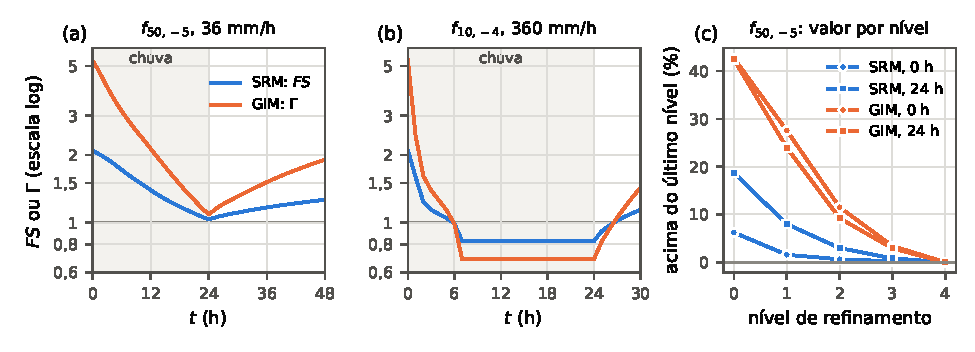
\includegraphics[width=\linewidth]{fig_gim_srm.pdf}
\caption{SRM e GIM: (a) f50 e (b) f10 no tempo, com $I = 1\,k_s$; (c) f50, valor de cada nível de refinamento acima do
valor do último nível, em 0 e 24~h.}\label{fig:gimsrm}
\end{figure}

Prós e contras:
\begin{itemize}
\item SRM. A favor: é o fator do Rahardjo (Bishop), o que permite a validação da Seção~\ref{sec:validacao}; converge
melhor com a malha e oscila menos; $FS$ é a margem de resistência, a leitura usual. Contra: custa o dobro, e a média e o
CoV de $FS$ não se comparam com os de $\Gamma$ nas tabelas do Ceron.
\item GIM. A favor: é mais barato, é a medida do Ceron e dá a mesma $P_f$. Contra: não tem referência na chuva (o
Rahardjo dá $FS$), infla longe da ruptura e converge pior com a malha.
\end{itemize}
\textbf{Escolha: SRM.} A $P_f$ é a mesma, e o SRM é o que tem referência e o que converge melhor. Para comparar médias e
CoV com o Ceron, basta rodar um caso à parte com \texttt{metodo=gim}.

\section{Intensidade da chuva}\label{sec:intensidade}
Com $I = 36$~mm/h (1~$k_s$), o $FS$ determinístico em 24~h é 1,0337 (\texttt{TriGMesh(2)}), quase 1. Para escolher a
intensidade de referência, o $FS$ determinístico em 24~h foi calculado de 18 a 36~mm/h (Tab.~\ref{tab:intensidade},
Fig.~\ref{fig:intensidade}a). O SRM fica de 1,1\% a 2,0\% abaixo da sigmoide ajustada na Fig.~7b do Rahardjo,
$F_{min}(I) = 0{,}82 + 1{,}83/\bigl(1 + e^{-(I - 10{,}7)/(-13{,}13)}\bigr)$.

A referência é $I = 31{,}05$~mm/h. Nela o GIM dá $\Gamma = 1{,}3345$, a $-0{,}1\%$ do $\Gamma = 1{,}336$ do determinístico
do Ceron (Fig.~24 do artigo). É a mesma margem determinística da referência do rebaixamento, na medida dele. Nessa
intensidade o SRM dá $FS = 1{,}1255$ (sigmoide: 1,140). A diferença para o 1,336 (0,0015) é bem menor que a oscilação
do GIM entre intensidades vizinhas (resíduo RMS de 0,0077).

\begin{table}[htbp]\centering\footnotesize
\caption{$f_{50,-5}$: $FS$ e $\Gamma$ determinísticos em 24~h com a intensidade (transiente em \texttt{TriGMesh(2)};
\texttt{mc/varre\_I*} e \texttt{mc/gim\_I/*}) e a sigmoide da Fig.~7b do Rahardjo.}\label{tab:intensidade}
\begin{tabular}{rrrrr}\toprule
$I$ (mm/h) & SRM: $FS$ & GIM: $\Gamma$ & sigmoide & SRM/sigmoide $- 1$ (\%) \\\midrule
18 & 1,4699 & -- & 1,487 & $-1{,}1$ \\
21 & 1,3731 & -- & 1,393 & $-1{,}5$ \\
24 & 1,2818 & -- & 1,308 & $-2{,}0$ \\
27 & 1,2060 & 1,5813 & 1,230 & $-2{,}0$ \\
30 & 1,1478 & 1,4003 & 1,162 & $-1{,}2$ \\
30,95 & 1,1293 & 1,3518 & 1,142 & $-1{,}2$ \\
31,05 & 1,1255 & 1,3345 & 1,140 & $-1{,}3$ \\
31,1 & 1,1222 & 1,3223 & 1,139 & $-1{,}5$ \\
31,3 & -- & 1,3078 & 1,135 & -- \\
33 & 1,0880 & -- & 1,103 & $-1{,}4$ \\
36 & 1,0337 & 1,0886 & 1,053 & $-1{,}8$ \\
\bottomrule\end{tabular}\end{table}

\begin{figure}[htbp]\centering
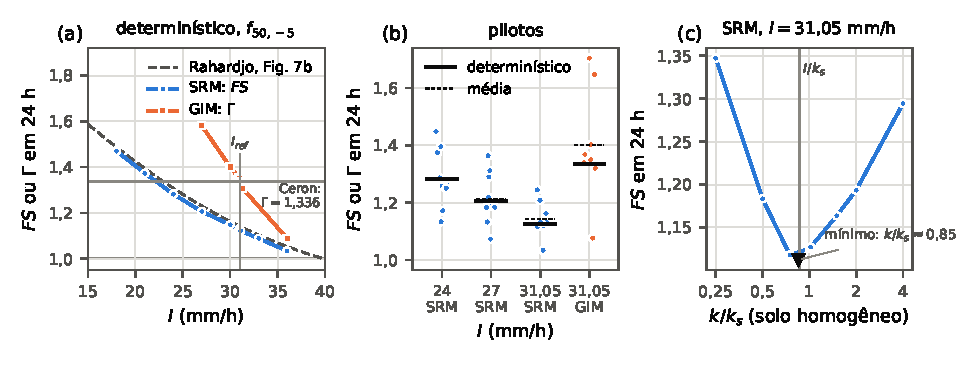
\includegraphics[width=\linewidth]{fig_intensidade.pdf}
\caption{(a) $FS$ e $\Gamma$ determinísticos em 24~h com $I$, a sigmoide da Fig.~7b do Rahardjo e o $\Gamma$ do
determinístico do Ceron; (b) pilotos em 24~h: cada ponto é uma realização (as mesmas sementes em todos), com o
determinístico e a média; (c) $FS$ em 24~h com $k/k_s$ no solo homogêneo ($c' = 10$~kPa, $\varphi' = 26^\circ$), com o
mínimo da parábola pelo ponto mais baixo e os seus dois vizinhos.}\label{fig:intensidade}
\end{figure}

\paragraph{Pilotos.} Os pilotos usam as realizações 0 a 9 (ou 0 a 7), as mesmas em todos os casos
(Tab.~\ref{tab:pilotos}, Fig.~\ref{fig:intensidade}b). Três observações:
\begin{itemize}
\item a média fica acima do determinístico: de $+0{,}2\%$ a $+1{,}6\%$ no SRM e $+5{,}0\%$ no GIM;
\item o CoV de $FS(24\text{ h})$ pelo SRM vai de 5,6\% a 7,6\% (o de $FS(0\text{ h})$ é 5,1\%), e o do GIM é 14,1\%. No
rebaixamento do Ceron, $CoV(\Gamma) = 23{,}5\%$: a chuva espalha o fator bem menos que o rebaixamento;
\item nenhuma realização rompeu. O ajuste log-normal dá $P_f$ de 0,05\% (24~mm/h) a 0,90\% (31,05~mm/h, SRM) e 1,03\%
(GIM). São estimativas grosseiras, com 8 a 10 realizações. A realização menos segura é a mesma pelos dois métodos (a 5).
\end{itemize}
Então a referência deve dar $P_f \approx 1\%$, e não os 11,5\% do Ceron: com a mesma margem determinística, a chuva
espalha menos o fator. Para ter $P_f$ maiores, a fase~3 da campanha vai até 45~mm/h.

\begin{table}[htbp]\centering\footnotesize\setlength{\tabcolsep}{3.5pt}
\caption{Pilotos ($f_{50,-5}$, \texttt{TriGMesh(2)} + \texttt{TriGMesh(1)} com 4 níveis). $n$: realizações; $FS_{det}$:
o determinístico do mesmo instante; $\Delta$: média$/FS_{det} - 1$; desvio e CoV amostrais; $n_f = \#(FS < 1)$; $P_f$
do ajuste log-normal, como no resumo do \texttt{SlopeRainMonteCarlo}.}\label{tab:pilotos}
\begin{tabular}{lrrrrrrrrr}\toprule
caso & $n$ & $FS_{det}$ & média & $\Delta$ (\%) & desvio & CoV (\%) & menor & $n_f$ & $P_f$ (\%) \\\midrule
SRM, $I = 24$, 0~h & 10 & 2,0939 & 2,1023 & 0,4 & 0,1066 & 5,1 & 1,8709 & 0 & 0,00 \\
SRM, $I = 24$, 24~h & 10 & 1,2818 & 1,2844 & 0,2 & 0,0976 & 7,6 & 1,1337 & 0 & 0,05 \\
SRM, $I = 27$, 24~h & 10 & 1,2060 & 1,2127 & 0,6 & 0,0868 & 7,2 & 1,0727 & 0 & 0,37 \\
SRM, $I = 31{,}05$, 24~h & 8 & 1,1255 & 1,1431 & 1,6 & 0,0637 & 5,6 & 1,0339 & 0 & 0,90 \\
GIM, $I = 31{,}05$, 24~h & 8 & 1,3345 & 1,4010 & 5,0 & 0,1972 & 14,1 & 1,0764 & 0 & 1,03 \\
\bottomrule\end{tabular}\end{table}

\paragraph{$FS$ e a permeabilidade.} Com o solo homogêneo ($c' = 10$~kPa, $\varphi' = 26^\circ$) e $I = 31{,}05$~mm/h, o
$FS(24\text{ h})$ tem um mínimo interior em $k$ (Fig.~\ref{fig:intensidade}c). Ele vale 1,3472 em $k/k_s = 0{,}25$,
1,1179 em 0,75 e 1,2944 em 4. A parábola pelo ponto mais baixo e os seus dois vizinhos ($k/k_s = 0{,}5$, 0,75 e 1) põe
o mínimo em $k/k_s \approx 0{,}85$ ($FS \approx 1{,}1121$), perto de $I/k_s = 0{,}863$. Com $k$ menor que $I$, a
superfície satura e a água que entra fica limitada por $k$. Com $k$ maior, a água entra toda, mas desce e escoa mais
rápido. Lembra a intensidade limiar do Rahardjo, vista pelo lado da permeabilidade (no f50, com $k$ fixo, ele acha
$I_{thr} = 51$~mm/h $= 1{,}42\,k_s$ na Fig.~7b). Duas consequências:
\begin{itemize}
\item a média $k/k_s = 1$ do determinístico fica perto do pior $k$, e a curva é em U em volta dela. A variação de $k$
sobe o $FS$ médio, o que é consistente com a média do Monte Carlo acima do determinístico;
\item no ponto de projeto do FORM, a derivada em $k$ é quase nula (Seção~\ref{sec:form}).
\end{itemize}

\section{FORM}\label{sec:form}
\subsection{Com variáveis aleatórias}
O \texttt{form\_variaveis.py} trata $c'$, $\varphi'$ e $k_s$ como variáveis log-normais, com as médias e os CoV dos
campos. O solo é homogêneo em cada avaliação, o que corresponde ao limite $s \to \infty$ dos campos. A função de estado
limite é $g = FS(24\text{ h}) - 1$, com $I = 31{,}05$~mm/h. O método é o HLRF, com o gradiente por diferenças centrais
com passo $h = 0{,}2$ no espaço normal padrão $u$; as 7 avaliações de cada iteração rodam em paralelo.

O resultado, em 5 iterações e 35 avaliações do $FS$ (Tab.~\ref{tab:form}):
\begin{itemize}
\item $\beta = 0{,}681$, então $P_f = \Phi(-\beta) = 24{,}8\%$;
\item ponto de projeto: $c' = 8{,}15$~kPa, $\varphi' = 24{,}85^\circ$ e $k/k_s = 0{,}853$;
\item importâncias $\alpha^2$: 0,637 ($c'$), 0,362 ($\varphi'$) e 0,000 ($k_s$).
\end{itemize}
Nas medianas ($u = 0$), $FS = 1{,}0937$. É menos que o 1,1255 das médias (Tab.~\ref{tab:intensidade}), porque as
medianas ficam abaixo delas. O passo
$h = 0{,}2$ muda $c'$ em 0,56~kPa e o $FS$ em 0,024. O ruído do $FS$ é de uns 0,001: com $c' = 10{,}1$ e 10,2~kPa, o $FS$
vale 1,1284 e 1,1323, saltos de 0,0028 e 0,0040 para o mesmo 0,1~kPa.

O $k$ do ponto de projeto oscila entre 0,83 e 0,85 de uma iteração para outra, e a derivada em $k$ fica entre 0,001 e
0,012. É o mínimo da Fig.~\ref{fig:intensidade}c: o ponto de projeto está no fundo da curva em $k$. Por isso
$\alpha_k^2 \approx 0$; o FORM lineariza e perde a curvatura em $k$, que um SORM levaria em conta.

\begin{table}[htbp]\centering\footnotesize
\caption{Iterações do FORM com variáveis aleatórias (\texttt{mc/form/trabalho\_I31.05/form.json}): $\beta = |u|$, o
ponto $x$, o $FS$ nele e o gradiente $\partial g/\partial u$ ($c'$, $\varphi'$, $k$).}\label{tab:form}
\begin{tabular}{rrrrrrl}\toprule
it. & $\beta$ & $c'$ (kPa) & $\varphi'$ (graus) & $k/k_s$ & $FS$ & $\partial g/\partial u$ \\\midrule
0 & 0,000 & 9,58 & 25,87 & 0,857 & 1,0937 & 0,120 0,079 0,012 \\
1 & 0,651 & 8,17 & 24,96 & 0,832 & 1,0047 & 0,110 0,075 0,001 \\
2 & 0,685 & 8,11 & 24,89 & 0,854 & 1,0016 & 0,108 0,076 0,010 \\
3 & 0,696 & 8,11 & 24,86 & 0,834 & 0,9983 & 0,101 0,074 0,002 \\
4 & 0,681 & 8,15 & 24,85 & 0,853 & 1,0021 & 0,108 0,081 0,003 \\
\bottomrule\end{tabular}\end{table}

A $P_f$ do FORM, 24,8\%, é a do solo homogêneo, muito acima do $\approx 1\%$ dos pilotos com $s = 1$. Linearizado nas
medianas, o desvio do $FS$ do solo homogêneo é $|\nabla g| = 0{,}144$, um CoV de uns 13\%, contra 5,6\% a 7,6\% nos
pilotos. Com $L_x = 20$~m e $L_y = 2$~m, a superfície de ruptura atravessa regiões fracas e fortes, e a média ao longo
dela espalha menos. No rebaixamento, o Ceron achou $P_f$ de 11,50\% em $s = 1$ e 21,93\% em $s = 400$. Na chuva, o FORM
e os pilotos sugerem uma diferença bem maior. O caso $s = 400$ da campanha confere o FORM: com 2000 realizações e $P_f \approx 25\%$,
$CoV(P_f) = 3{,}9\%$.

\subsection{Com campos aleatórios}
Com campos, as variáveis do FORM são os coeficientes da KL: $3m$ para $m$ termos por campo. Com diferenças centrais, cada
iteração custa $2 \cdot 3m + 1$ avaliações do $FS$: 301 com $m = 50$, 1201 com $m = 200$ e 12\,001 com $m = 2000$. Com as
5 iterações do caso das variáveis, seriam 1505 avaliações com $m = 50$ e 6005 com $m = 200$; a referência do Monte
Carlo tem 5000 realizações. A truncagem perde variância
(Tab.~\ref{tab:kl}): em $s = 1$, 50 termos retêm 64,5\% e 200 termos, 83,4\%; os 2000 da campanha retêm 96,4\%.

\begin{table}[htbp]\centering\footnotesize
\caption{Variância retida (\%) pelos $m$ maiores termos da KL com correlação exponencial separável no retângulo de 70~m
$\times$ 30~m (as formas fechadas do \texttt{KLSeparavel.h}).}\label{tab:kl}
\begin{tabular}{rlrrrrrrrr}\toprule
$s$ & $L_x \times L_y$ (m) & $m = 10$ & 20 & 50 & 100 & 200 & 500 & 1000 & 2000 \\\midrule
1 & 20~$\times$~2 & 33,3 & 47,0 & 64,5 & 75,3 & 83,4 & 90,7 & 94,1 & 96,4 \\
2 & 40~$\times$~4 & 57,8 & 70,1 & 82,4 & 88,6 & 92,8 & 96,2 & 97,7 & 98,6 \\
5 & 100~$\times$~10 & 81,9 & 88,6 & 94,0 & 96,4 & 97,8 & 98,9 & 99,4 & 99,6 \\
\bottomrule\end{tabular}\end{table}

O que a literatura usa:
\begin{itemize}
\item Siacara, Beck e Futai (2020) acoplam o FORM direto à percolação transiente e ao equilíbrio limite no rebaixamento de
uma barragem, com variáveis aleatórias.
\item Liao e Ji (2021) fazem o FORM com um campo de $k_s$ por KL sob chuva, com $\beta$ em instantes discretos.
\item Ji, Liao, Hu e Lü (2024) truncam a KL, acham o ponto de projeto pelo FORM com elementos finitos e corrigem a $P_f$
por amostragem por importância em torno dele, porque o FORM sozinho não basta em alta dimensão.
\item Santoso, Phoon e Quek (2011) usam simulação por subconjuntos com um campo log-normal de $k_s$ sob chuva, o que
serve para $P_f$ pequenas.
\end{itemize}
Há duas opções para os campos: (i) KL truncada (50 a 200 termos) com amostragem por importância centrada no ponto de
projeto; (ii) simulação por subconjuntos na KL inteira, sem truncar. Para a campanha fica o Monte Carlo: a $P_f$ esperada
vai de 1\% a dezenas de por cento, e as realizações são independentes, o que paraleliza sem perda no fermi. O ganho do
FORM é o ponto de projeto e as importâncias. A Seção~\ref{sec:ai} mostra uma terceira opção: a amostragem por
importância sem o ponto de projeto, com o deslocamento tirado das falhas de um piloto.

\section{Amostragem por importância}\label{sec:ai}
A $P_f$ é uma integral em $n = 6000$ dimensões: os coeficientes $\xi$ da KL dos três campos, 2000 por campo. Cada ponto
da integral é uma análise por elementos finitos. Há três maneiras de calculá-la: Monte Carlo direto, FORM e amostragem
por importância (AI). A Tab.~\ref{tab:metodos} resume as três. Esta seção explica a AI, por que ela entra no estudo e
como ela foi testada no rebaixamento rápido do Ceron com o transiente (\texttt{rebaixamento\_mc.cpp}), onde há um
Monte Carlo direto para comparar.

\begin{table}[htbp]\centering\footnotesize
\caption{Os três métodos para a $P_f$ com $n = 6000$ variáveis (os $\xi$ da KL), com uma análise por elementos finitos
em cada avaliação. Os números de realizações são para $CoV(P_f) = 5\%$.}\label{tab:metodos}
\newcolumntype{L}[1]{>{\raggedright\arraybackslash}p{#1}}
\begin{tabular}{@{}L{1.9cm}L{3.5cm}L{4.6cm}L{5.3cm}@{}}\toprule
Método & Custo & Vantagens & Desvantagens \\\midrule
Monte Carlo direto & $N \approx (1 - P_f)/(0{,}0025\,P_f)$: 1762 com $P_f = 18{,}5\%$ e 39\,600 com 1\% &
sem viés e sem hipótese sobre a região de falha; vale com vários mecanismos; paraleliza sem perda; dá também a
distribuição de $\Gamma$ e os mecanismos & o custo cresce com $1/P_f$ \\\addlinespace
FORM & $2n + 1$ análises por iteração: 7 com 3 variáveis, 12\,001 com os campos & ponto de projeto e importâncias
$\alpha^2$; barato com poucas variáveis & erro da linearização sem estimativa; um ponto de projeto só; diferenças
finitas sobre o ruído do $FS$; inviável com 6000 variáveis \\\addlinespace
Amostragem por importância & um piloto e de 3,5 a 288 vezes menos realizações que o direto
(Tab.~\ref{tab:ganho}) & sem viés com o peso exato; não precisa de gradiente; ganho grande com $P_f$ pequena; o mesmo
peso em todos os instantes & precisa de um piloto com falhas; o deslocamento tem de estar certo e sem ruído; um
mecanismo longe do deslocamento aumenta a variância \\
\bottomrule\end{tabular}\end{table}

\subsection{Monte Carlo direto e FORM}
O Monte Carlo direto sorteia $\xi \sim N(0, I)$ e conta as falhas: $\hat P_f = n_f/N$, com
$CoV(\hat P_f) = \sqrt{(1 - P_f)/(N P_f)}$ (Eq.~68 do Ceron).
\begin{itemize}
\item \textbf{Vantagens:}
  \begin{itemize}
  \item não tem viés nem hipótese sobre a região de falha: vale com vários mecanismos e com um $FS$ não linear e com
  ruído;
  \item as realizações são independentes e paralelizam sem perda;
  \item além da $P_f$, dá a distribuição de $\Gamma$, os mecanismos e as correlações (Spearman, mapa da banda).
  \end{itemize}
\item \textbf{Desvantagem:} o custo cresce com $1/P_f$. Para $CoV(P_f) = 5\%$ são precisas
$N \approx (1 - P_f)/(0{,}0025\,P_f)$ realizações: 1762 com $P_f = 18{,}5\%$, 39\,600 com 1\% e 399\,600 com 0,1\%
(Tab.~\ref{tab:ganho}).
\end{itemize}

O FORM troca a integral pelo ponto de projeto $u^*$, o ponto da superfície de falha mais perto da origem, e dá
$P_f \approx \Phi(-\beta)$, com $\beta = |u^*|$ (Seção~\ref{sec:form}).
\begin{itemize}
\item \textbf{Vantagens:} com poucas variáveis, é barato (35 avaliações na Seção~\ref{sec:form}); dá o ponto de
projeto e as importâncias $\alpha^2$, que dizem qual variável pesa.
\item \textbf{Desvantagens:}
  \begin{itemize}
  \item o gradiente por diferenças centrais custa $2n + 1 = 12\,001$ análises por iteração com $n = 6000$, mais que o
  Monte Carlo inteiro da referência;
  \item o $FS$ tem ruído de uns 0,001 (a tolerância do método e a malha adaptativa, que muda de uma avaliação para
  outra), o que pede passos grandes nas diferenças;
  \item o erro da linearização não tem estimativa: na Seção~\ref{sec:form}, o mínimo do $FS$ em $k$ deu
  $\alpha_k^2 \approx 0$, embora $k$ mude o $FS$;
  \item há um ponto de projeto só: um segundo mecanismo, com outra superfície de ruptura, fica de fora.
  \end{itemize}
\end{itemize}

\subsection{O estimador da amostragem por importância}
A AI sorteia os $\xi$ de outra densidade, a normal deslocada $h(\xi) = \varphi_n(\xi - \mu)$, mais perto da falha, e
corrige cada realização com um peso:
\begin{equation}
P_f = \int I[\Gamma(\xi) < 1]\, \varphi_n(\xi)\, d\xi = \mathrm{E}_h\big[I\, w\big], \qquad
w(\xi) = \frac{\varphi_n(\xi)}{\varphi_n(\xi - \mu)} = \exp\!\big(-\xi \cdot \mu + \tfrac12 |\mu|^2\big),
\end{equation}
\begin{equation}
\hat P_f = \frac1N \sum_{i=1}^N I_i\, w_i, \qquad CoV(\hat P_f) = \frac{s_q}{\sqrt N\, \hat P_f},
\end{equation}
com $s_q$ o desvio padrão amostral de $q_i = I_i w_i$.

\paragraph{Não há viés.} A primeira igualdade é uma troca de variável exata, e $h > 0$ em todo o espaço: a média de
$\hat P_f$ é $P_f$ para qualquer $\mu$. O $\mu$ só muda a variância. Duas condições garantem isso no programa:
\begin{itemize}
\item o peso é o exato, calculado com o $\mu$ usado no sorteio (coluna \texttt{log\_peso});
\item o $\mu$ é fixado antes da amostra e não depende dela: ele sai de um piloto, com outra semente.
\end{itemize}
A conferência usa 20\,000 sorteios sem elementos finitos (\path|verificacao/|):
\begin{itemize}
\item a média dos pesos é $1{,}007 \pm 0{,}020$ com o deslocamento na banda e $1{,}008 \pm 0{,}020$ com o
deslocamento por modos;
\item a variância deles é 8,21 e 8,07, contra $e^{|\mu|^2} - 1 = 7{,}54$ e 7,59;
\item a média das projeções sorteadas, $(-1{,}23;\ -0{,}60;\ -0{,}52)$, é o deslocamento pedido.
\end{itemize}

\paragraph{Alta dimensão.} Com $\xi \sim h$, $\mathrm{E}_h[w^2] = e^{|\mu|^2}$, qualquer que seja $n$: a AI funciona com
6000 variáveis se o deslocamento for o certo. Um deslocamento com ruído $\delta$ em direções que não importam
multiplica o segundo momento por $e^{|\delta|^2}$ (Au e Beck, 2003). Por isso a covariância de $h$ fica a identidade, e
o deslocamento tem de ter poucos graus de liberdade.

\subsection{O deslocamento sem gradiente: entropia cruzada}
Entre as normais $N(\mu, I)$, a melhor no sentido da entropia cruzada (Rubinstein e Kroese, 2004) tem
$\mu^* = \mathrm{E}[\xi \mid \Gamma < 1]$, a média dos $\xi$ das realizações que falham. Ela sai de um piloto de Monte
Carlo direto; os $\xi$ das falhas são sorteados de novo pela semente, sem custo. A média crua dos 6000 componentes
teria ruído $|\delta|^2 \approx 6000/n_f$. O programa a regulariza de dois jeitos (\texttt{ai=banda} ou
\texttt{ai=modos}):
\begin{itemize}
\item \textbf{Na direção da banda.} $d$ é o vetor unitário do gradiente, em relação aos $\xi$, da média do campo
gaussiano nos pontos da banda de ruptura do determinístico. O deslocamento é $\mu_c = s_c\, d$, com $s_c$ a média de
$\xi_c \cdot d$ nas falhas: três números, um por campo, e ruído $3/n_f$.
\item \textbf{Nos primeiros modos.} A média dos $K = 20$ primeiros modos de cada campo (a proposta da nota
\texttt{form\_MIS}): 60 números e ruído $60/n_f$. Ela só alcança a parte da direção útil que está nesses modos: 65\% de
$|d|^2$.
\end{itemize}
O ponto de projeto do FORM também serviria de $\mu$, como em Ji et al.\ (2024); aqui ele custaria as iterações do
gradiente, e um ponto de projeto impreciso põe ruído no deslocamento.

\paragraph{O piloto do rebaixamento.} As 400 primeiras realizações do Monte Carlo direto no PC têm 74 falhas
($P_f = 18{,}5\%$).
\begin{itemize}
\item O deslocamento na banda é $s = (-1{,}22;\ -0{,}62;\ -0{,}52)$ para $c'$, $\varphi'$ e $k_v$
(Fig.~\ref{fig:ai}b). As falhas têm $c'$, $\varphi'$ e $k_v$ menores ao longo da banda: uma banda mais fraca e uma
dissipação mais lenta da pressão da água depois do rebaixamento.
\item $|\mu|^2 = 2{,}15$, perto do $m^2 = 2{,}08$ de um estado limite linear com a mesma $P_f$ (Tab.~\ref{tab:ganho}):
a direção da banda explica a falha.
\item Com 74 falhas, o ruído é $3/n_f = 0{,}04$ na banda e $60/n_f = 0{,}81$ por modos. No piloto do fermi (1000
realizações, umas 185 falhas), o ruído por modos cai para 0,32, um fator $e^{0{,}32} = 1{,}38$ no segundo momento.
\end{itemize}

\begin{figure}[htbp]\centering
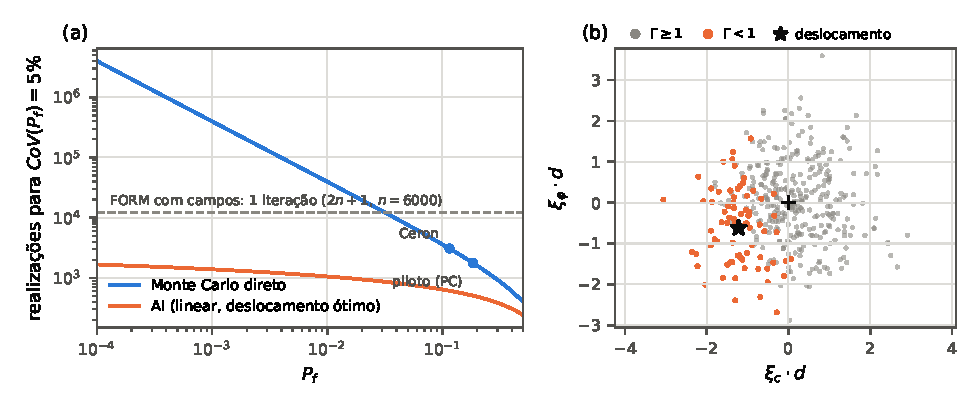
\includegraphics[width=\linewidth]{fig_ai.pdf}
\caption{(a) Realizações para $CoV(P_f) = 5\%$ pelo Monte Carlo direto e pela AI num estado limite linear com o
deslocamento ótimo. A linha tracejada é uma iteração do FORM com os campos. Os pontos são a $P_f$ do piloto do
rebaixamento e a do Ceron. (b) O piloto do rebaixamento (400 realizações) no plano das projeções na direção da banda,
$\xi_c \cdot d$ e $\xi_\varphi \cdot d$: as falhas ($\Gamma < 1$) e o deslocamento $(s_c, s_\varphi)$.}\label{fig:ai}
\end{figure}

\subsection{O ganho esperado}
Num estado limite linear, o deslocamento ótimo da entropia cruzada é $m = \varphi(\beta)/P_f$ na direção da falha. O
segundo momento é então $e^{m^2}\Phi(-\beta - m)$, e a razão das variâncias por realização sai em forma fechada
(Tab.~\ref{tab:ganho} e Fig.~\ref{fig:ai}a). É o melhor caso: o $\Gamma$ não é linear, e a direção da banda é uma
aproximação.
\begin{itemize}
\item Com $P_f = 18{,}5\%$, a AI precisa de 505 realizações em vez de 1762 para $CoV(P_f) = 5\%$: 3,5 vezes menos.
\item Com $P_f = 1\%$, 1057 em vez de 39\,600 (37,5 vezes); com 0,1\%, 1388 em vez de 399\,600 (288 vezes).
\end{itemize}
Com a $P_f$ da referência, o ganho é modesto, e o Monte Carlo direto basta. A AI compensa quando a $P_f$ é pequena:
\begin{itemize}
\item casos de sensibilidade com CoV pequeno ou intensidades menores;
\item o começo da curva $P_f(t)$ da chuva;
\item probabilidades de projeto.
\end{itemize}
Na chuva há mais uma vantagem: o peso não depende do instante, então uma amostra dá $P_f(t)$ em todos eles.

\begin{table}[htbp]\centering\footnotesize
\caption{Ganho da AI num estado limite linear com o deslocamento ótimo da entropia cruzada: $\beta$, $m^2 = |\mu|^2$,
realizações para $CoV(P_f) = 5\%$ pelo Monte Carlo direto e pela AI, e a razão entre elas.}\label{tab:ganho}
\begin{tabular}{rlrrrrr}\toprule
$P_f$ (\%) & & $\beta$ & $m^2$ & $N$ direto & $N$ AI & razão \\\midrule
18,5 & piloto do rebaixamento (PC) & 0,90 & 2,08 & 1762 & 505 & 3,5 \\
11,5 & Ceron, Tabela 4 & 1,20 & 2,85 & 3078 & 612 & 5,0 \\
1,0 &  & 2,33 & 7,10 & 39\,600 & 1057 & 37,5 \\
0,10 &  & 3,09 & 11,34 & 399\,600 & 1388 & 288 \\
\bottomrule\end{tabular}\end{table}

\paragraph{O risco.} Se a região de falha tem uma parte longe do deslocamento (outro mecanismo), o estimador continua
sem viés, mas essa parte aparece pouco e com pesos grandes. A variância sobe e, com $N$ finito, a $P_f$ tende a sair
baixa. Por isso a AI é conferida contra o Monte Carlo direto e acompanhada pelo tamanho efetivo da amostra.

\subsection{Teste no rebaixamento do Ceron}
O Monte Carlo direto do rebaixamento com o transiente dá, nas 400 primeiras realizações:
\begin{itemize}
\item $P_f = 18{,}5\%$ (IC 95\%: 14,7 a 22,3\%), contra 11,50\% do Ceron;
\item $\bar\Gamma = 1{,}278$ e $CoV(\Gamma) = 24{,}3\%$, contra o CoV de 23,5\% do Ceron;
\item $\Gamma = 1{,}3253$ no determinístico, contra 1,336 do Ceron.
\end{itemize}
O transiente baixa a média de $\Gamma$, e a dispersão fica a mesma. A diferença de $P_f$ ainda será conferida com mais
realizações.

Duas rodadas comparam a AI com o Monte Carlo direto:
\begin{itemize}
\item \textbf{PC:} 2000 realizações diretas e, depois, 1000 com cada deslocamento, calculado pelas 2000.
\item \textbf{fermi} (\texttt{cluster/casos\_ceron.txt}, \texttt{CAMPANHA=ceron}): 10\,000 realizações diretas e
5000 com cada deslocamento, com sementes diferentes.
  \begin{itemize}
  \item As AI começam quando as realizações 0 a 999 do direto, o piloto, terminam, e cada bloco calcula o mesmo
  deslocamento.
  \item São umas 481~h de CPU (33~s por realização no PC, com 8 processos, e 2,6 vezes isso no fermi): cerca de 10~h com 4 nós.
  \end{itemize}
\end{itemize}
O resultado esperado tem duas partes:
\begin{itemize}
\item a conferência do viés: as $P_f$ da AI dentro de dois desvios da $P_f$ do direto;
\item o ganho medido: quantas realizações diretas dão o mesmo CoV que as da AI.
\end{itemize}

\subsection{Quando usar cada um}
\begin{itemize}
\item \textbf{$P_f \gtrsim 5\%$ (a referência):} Monte Carlo direto. A AI ganha de 3 a 5 vezes, se o deslocamento
estiver certo.
\item \textbf{$P_f \lesssim 1\%$:} AI com o deslocamento pela entropia cruzada na direção da banda, com ganho de
dezenas a centenas de vezes.
  \begin{itemize}
  \item Se o piloto tiver poucas falhas, o conjunto elite são os 10\% de menor $\Gamma$, um nível intermediário (opção
  \texttt{elite}).
  \item Com mecanismos múltiplos, a simulação por subconjuntos (Santoso et al., 2011) não precisa de deslocamento.
  \end{itemize}
\item \textbf{FORM:} com poucas variáveis aleatórias, para o ponto de projeto e as importâncias
(Seção~\ref{sec:form}). Com campos, só com a KL truncada e como ponto de partida.
\end{itemize}


\section{Campanha no fermi}\label{sec:fermi}
\subsection{Casos e custo}
Os casos estão em \texttt{cluster/casos.txt} (Tab.~\ref{tab:casos}): 27 casos e 57\,000 realizações. A referência
($I = 31{,}05$~mm/h) tem 5000 realizações, com o $FS$ em 0, 6, 12, 18 e 24~h: o $FS$ em $t$ é o do fim de uma chuva de
$t$ horas. Os outros casos têm 2000 realizações, com o $FS$ em 24~h e também em 0~h onde $c'$ ou $\varphi'$ mudam. O
bloco de cada caso que começa na realização 0 roda também o determinístico e grava os campos dele.

O custo vem de uma realização em série na estação (\texttt{mc/serial\_I24.log}): 116,5~s, sendo 34,3~s do transiente e
41,1~s por instante do SRM adaptativo. Isso dá 75,4~s com um instante, 116,5~s com dois e 239,8~s com cinco. Um núcleo
do fermi é 2,6 vezes mais lento. A estimativa é conservadora para os casos só com 24~h: nessa realização o SRM levou
20,4~s em 24~h e 61,8~s em 0~h.

\begin{table}[htbp]\centering\footnotesize\setlength{\tabcolsep}{4pt}
\caption{Casos da campanha (\texttt{cluster/casos.txt}), por família: $N$ é o número de realizações de cada caso (nas
linhas das fases, o total). Custo por realização em série na estação; horas de CPU no fermi (2,6 vezes a estação) e
horas de relógio com 4 nós $\times$ 12 processos.}\label{tab:casos}
\begin{tabular}{rlllrrrr}\toprule
fase & família & valores & $N$ & instantes (h) & s/realização & CPU (h) & relógio (h) \\\midrule
1 & referência & $I = 31{,}05$~mm/h & 5000 & 0, 6, 12, 18, 24 & 239,8 & 866 & 18,0 \\
2 & $CoV(k_s)$ & 0, 0{,}75, 0{,}9, 1 & 2000 & 24 & 75,4 & 436 & 9,1 \\
2 & $CoV(c')$ & 0{,}1, 0{,}5, 0{,}7 & 2000 & 0, 24 & 116,5 & 505 & 10,5 \\
2 & $CoV(\varphi')$ & 0{,}05, 0{,}15, 0{,}2 & 2000 & 0, 24 & 116,5 & 505 & 10,5 \\
2 & $s$ & 1{,}5, 2, 5, 10, 20, 400 & 2000 & 0, 24 & 116,5 & 1010 & 21,0 \\
2 & $\alpha = k_h/k_v$ & 2, 3, 4, 5 & 2000 & 24 & 75,4 & 436 & 9,1 \\
3 & $I$ (mm/h) & 24, 27, 29, 33, 36, 45 & 2000 & 24 & 75,4 & 653 & 13,6 \\
\midrule
\multicolumn{3}{l}{fase 1} & 5000 & & & 866 & 18,0 \\
\multicolumn{3}{l}{fase 2} & 40000 & & & 2891 & 60,2 \\
\multicolumn{3}{l}{fase 3} & 12000 & & & 653 & 13,6 \\
\multicolumn{3}{l}{total} & 57000 & & & 4410 & 91,9 \\
\bottomrule\end{tabular}\end{table}

Com 4 nós de 12 processos (o fermi deixa rodar 4 jobs por usuário), a campanha leva uns 3,8 dias: 18,0~h na fase~1,
60,2~h na fase~2 e 13,6~h na fase~3. Cada job tem o limite padrão de 2 dias (\texttt{2-00:00:00}), então a campanha
inteira pede pelo menos uma ressubmissão, que retoma de onde parou. A precisão segue a Eq.~68 do Ceron,
$CoV(P_f) = \sqrt{(1 - P_f)/(N P_f)}$. Com $P_f = 1\%$, o CoV é 14\% na referência ($N = 5000$) e 22\% nos casos de 2000.
Com $P_f = 10\%$, é 4\% e 7\%.

\subsection{O que cada realização grava}
Uma linha por realização e instante em \texttt{mc\_<a>\_<z>.csv}, com os nomes do \texttt{mc\_resumo.csv} do
rebaixamento onde existem:
\begin{itemize}
\item \texttt{FS\_min}, \texttt{situacao} e \texttt{niveis} (o $FS$ de cada nível do refinamento);
\item a banda de ruptura (\texttt{banda\_*}, $\sqrt{J_2(\varepsilon_p)} \geq 0{,}1$ do maior): área, profundidade,
extensão, centroide e as médias de $p_w$, $c'$, $\varphi'$ e $k$ nela;
\item a massa que desliza (\texttt{massa\_*}, $|\Delta u|$ desde o estado geostático $\geq 0{,}5$ do maior): área,
centroide, $c'$, $\varphi'$ e $k$;
\item as médias dos campos no solo todo e a cota do nível d'água na crista, no meio da face e no pé ($x = 30$, 35 e
40~m), para as categorias I a IV da Tabela~3 do Rahardjo;
\item faixa de $p_w$, nós na face de percolação, equações e tempos, e os parâmetros do caso.
\end{itemize}
O \texttt{mc\_mapa\_<a>\_<z>.csv} conta, em células de 1~m e em cada instante, as realizações com a banda ali e quantas
delas romperam. A pasta \texttt{mc\_real-1/} guarda os campos do determinístico.

\subsection{Pós-processamento}
O \texttt{cluster/baixar.sh} roda no PC. Ele baixa \path|$DATA/chuva_mc| para \path|~/projects/runs/fermi_chuva| e
roda o \texttt{posproc/}:
\begin{itemize}
\item \texttt{dados\_chuva.py}: por caso e instante, $S$, $n_f$, $P_f$, $CoV(P_f)$, intervalo de Wilson, ajuste
log-normal ($\mu$, mediana, $\sigma$, CoV, como nas tabelas do Ceron), qui-quadrado, convergência de $P_f$, Spearman
parcial de 2ª ordem (Eqs.~70 e 71), curva da duração, pares $FS(0)$ e $FS(24\text{ h})$, mapa da banda e categorias do
nível d'água;
\item \texttt{figuras\_chuva.py}: as análogas das Figs.~24 a 33 do Ceron, mais a duração, $FS(0) \times FS(24\text{ h})$,
o mapa da banda e as categorias do nível;
\item \texttt{relatorio\_chuva.py}: o relatório em PDF.
\end{itemize}
O pós-processamento foi testado em 7 casos de 8 realizações (\texttt{mc/teste\_casos}), num relatório de 13 páginas.

\subsection{Como rodar}
Os comandos estão no \texttt{cluster/README.md}, todos rodados do PC com a VPN da UFRGS ligada. Em resumo:
\begin{enumerate}
\item mandar o código (\texttt{git push}) e atualizar o fermi (\texttt{git pull});
\item compilar no nó de login com \texttt{./compilar.sh}, em segundo plano;
\item conferir o ambiente com \texttt{sbatch teste.sbatch}. O determinístico deve dar $FS(0) \approx 2{,}094$ e
$FS(24\text{ h}) \approx 1{,}126$;
\item submeter: \texttt{./submeter.sh 4}; só a referência: \texttt{CASOS=fase1 ./submeter.sh 4};
\item acompanhar com \texttt{status.sh}, baixar e gerar o relatório com \texttt{baixar.sh}.
\end{enumerate}
Parar, retomar e estender estão no README: as tarefas feitas são puladas, e as interrompidas são refeitas.

\section{Próximos passos}\label{sec:proximos}
\begin{itemize}
\item Rodar a fase~1 e conferir, no relatório parcial, a $P_f$ da referência e o CoV de $FS$ contra os pilotos.
\item Estender $N$ onde a $P_f$ for pequena. Para $CoV(P_f) = 5\%$ com $P_f = 1\%$ são precisas 39\,600 realizações
(com 10\%, 3600), o que fica caro. Para $P_f$ pequenas, as alternativas são a amostragem por importância
(Seção~\ref{sec:ai}) e a simulação por subconjuntos (Santoso et al., 2011).
\item Comparar o caso $s = 400$ com o FORM ($P_f = 24{,}8\%$) e, se a diferença pedir, fazer o SORM em $k$.
\item Concluir a comparação da amostragem por importância com o Monte Carlo direto no rebaixamento (PC e fermi) e
usá-la nos casos da chuva com $P_f$ pequena, com um piloto por caso (\texttt{piloto=} no \texttt{casos.txt}).
\item Ar ativo: o material já tem $p_a$; o transiente atual usa ar passivo ($p_a = 0$), como o SEEP/W do artigo.
\end{itemize}

\appendix
\section{Arquivos lidos}\label{sec:arquivos}
\sloppy Os caminhos são relativos à pasta do build do projeto, a do executável \texttt{SlopeRainMonteCarlo}. Das
fontes são lidos \texttt{montecarlo.cpp}, \texttt{RainTransient.h}, \texttt{casos.txt}, \texttt{casos\_ceron.txt},
\texttt{campanha.sh}, \texttt{submeter.sh}, \texttt{job.sbatch} e \texttt{teste.sbatch}.
\begin{itemize}\small
\item Seção~\ref{sec:modelo}: \path|mc/valida_0_-1.csv|, \path|mc/semchuva_0_-1.csv|, \path|mc/varre_I36_0_-1.csv|,
\path|mc/teste_casos/ref/mc_real-1/| (malha), \path|mc/gim_I/gim_I31.05_parametros.txt|.
\item Seção~\ref{sec:validacao}: \path|rahardjo_f10.log|, \path|rahardjo_f50.log|, \path|rahardjo_f100.log|,
\path|f50/chuva_f50_36/| (Fig.~\ref{fig:estado}), \path|mc/semchuva_0_-1.csv|.
\item Seção~\ref{sec:gimsrm}: \path|gim_f50.log|, \path|gim_f10.log|, \path|srm_f50_6h_sozinho.log| e os
\path|rahardjo_f*.log|.
\item Seção~\ref{sec:intensidade}: \path|mc/varre_I*_0_-1.csv| (18 a 36~mm/h), \path|mc/gim_I/gim_I*_0_-1.csv|,
\path|mc/gim_I/srm_I*_0_-1.csv|, \path|mc/piloto_I24_0_9.csv|, \path|mc/piloto_I27_0_9.csv|,
\path|mc/gim_I/piloto_srm_I31.05_0_7.csv|, \path|mc/gim_I/piloto_gim_I31.05_0_7.csv|,
\path|mc/form/v_<c>,<phi>,<k>_0_-1.csv|.
\item Seção~\ref{sec:form}: \path|mc/form/trabalho_I31.05/form.json|, \path|mc/form/v_10.1,26,1_0_-1.csv| e
\path|mc/form/v_10.2,26,1_0_-1.csv|; a Tab.~\ref{tab:kl} é calculada.
\item Seção~\ref{sec:ai}: na pasta \path|~/projects/runs/ceron_transiente|, as realizações 0 a 399 de
\path|direto/ceron_tr_fase1/f50_I0_iii/mc_*.csv| (o piloto), \path|verificacao/banda_*| e \path|verificacao/modos_*|
(os sorteios com os pesos, \path|verificacao/LEIAME.txt|) e \path|verificacao/banda_direcao.csv|; das fontes,
\texttt{cluster/casos\_ceron.txt}. A Tab.~\ref{tab:ganho} é calculada.
\item Seção~\ref{sec:fermi}: \texttt{casos.txt}, \texttt{campanha.sh}, \texttt{submeter.sh}, \texttt{job.sbatch},
\texttt{teste.sbatch}, \path|mc/serial_I24.log|,
\path|mc/serial_I24_0_0.csv|.
\end{itemize}
Digitados no script: as leituras da Fig.~5, o $F_{ini}$ da Tabela~7, a sigmoide e o $I_{thr}$ da Fig.~7b do Rahardjo; o
$\Gamma$
determinístico (Fig.~24), os $P_f$ e o $CoV(\Gamma)$ da Tabela~4 do Ceron; e o fator 2,6 entre os núcleos do fermi e da
estação.

\begin{thebibliography}{9}
\bibitem{au2003} Au e Beck (2003). Importance sampling in high dimensions. \emph{Structural Safety} 25(2):139--163.
doi:10.1016/S0167-4730(02)00047-4.
\bibitem{ji2024} Ji, Liao, Hu e Lü (2024). Integrated reliability analysis procedure for spatially variable soil slopes
using recursive FORM algorithm enhanced by importance sampling: Abaqus via Python implementations. \emph{Georisk}
18(2):346--360. doi:10.1080/17499518.2023.2283857.
\bibitem{liao2021} Liao e Ji (2021). Time-dependent reliability analysis of rainfall-induced shallow landslides
considering spatial variability of soil permeability. \emph{Computers and Geotechnics} 129:103903.
doi:10.1016/j.compgeo.2020.103903.
\bibitem{rahardjo2007} Rahardjo, Ong, Rezaur e Leong (2007). Factors controlling instability of homogeneous soil slopes
under rainfall. \emph{Journal of Geotechnical and Geoenvironmental Engineering} 133(12):1532--1543.
doi:10.1061/(ASCE)1090-0241(2007)133:12(1532).
\bibitem{rubinstein2004} Rubinstein e Kroese (2004). \emph{The Cross-Entropy Method}. Springer, Nova York.
doi:10.1007/978-1-4757-4321-0.
\bibitem{santoso2011} Santoso, Phoon e Quek (2011). Effects of soil spatial variability on rainfall-induced landslides.
\emph{Computers \& Structures} 89(11--12):893--900. doi:10.1016/j.compstruc.2011.02.016.
\bibitem{siacara2020} Siacara, Beck e Futai (2020). Reliability analysis of rapid drawdown of an earth dam using direct
coupling. \emph{Computers and Geotechnics} 118:103336. doi:10.1016/j.compgeo.2019.103336.
\bibitem{ceron2025} Vargas Ceron, Cecílio, Linn e Maghous (2025). Stability analysis of slope subjected to seepage forces
considering spatial variability of soil properties. \emph{International Journal for Numerical and Analytical Methods in
Geomechanics} 49(11):2459--2491. doi:10.1002/nag.3993.
\end{thebibliography}
\end{document}
